\documentclass[12pt, letterpaper]{memoir}
\usepackage{ExamStyle}

\begin{document}
	\pagestyle{empty}
	\begin{center}
		{\Huge Rowley CHEM 1220 Midterm 4}
	\end{center}

	{\large Formulas}

	\begin{minipage}{0.5\linewidth}
		$S=k_B\ln W$

    $\Delta S_{universe} = \Delta S_{sys} + \Delta S_{surr}$

    $\Delta G = \Delta H - T\Delta S$

    $\Delta G = \Delta G^{\circ} + RT\ln Q$

    $E^\circ_{cell}=E^\circ_{cathode}-E^\circ_{anode}$

    $\Delta G^\circ = -nFE^\circ$

    $E^\circ = \dfrac{RT}{nF}\ln K$

    $\dfrac{N}{N_0}=\left(\dfrac{1}{2}\right)^{\frac{t}{t_{\nicefrac{1}{2}}}}$

	\end{minipage}
	\begin{minipage}{0.5\linewidth}
		$\displaystyle\Delta S^{\circ}_{rxn} = \sum\limits_{i, products} \nu_iS_i^{\circ} - \sum_{j, reactants} \nu_jS_j^{\circ}$

    $\Delta S_{surr} = \dfrac{-q_sys}{T}$

    $\Delta G^\circ = \Delta H^\circ - T\Delta S^\circ$

    $\Delta G^{\circ} = -RT\ln K$

    $\dfrac{C_1V_1}{n_1}=\dfrac{C_2V_2}{n_2}$

    $\Delta G=-nFE$

    $E = E^\circ - \dfrac{RT}{nF}\ln Q$

    $E=mc^2$
	\end{minipage}

	\vspace{2em}

	{\large Constants}

	$R=8.314 \dfrac{J}{mol~K}$

	$R=0.08206 \dfrac{L~atm}{mol~K}$

	$k_B=1.380649 \times 10^{-23} \dfrac{J}{K}$

	$N_A=6.022\times10^{23}mol^{-1}$

  $F=96,485~\dfrac{C}{mol}$

  $c=2.998\times10^8\frac{m}{s}$

    \newgeometry{top=1mm, bottom=1mm, left=1mm, right=1mm}


\hspace{6em}	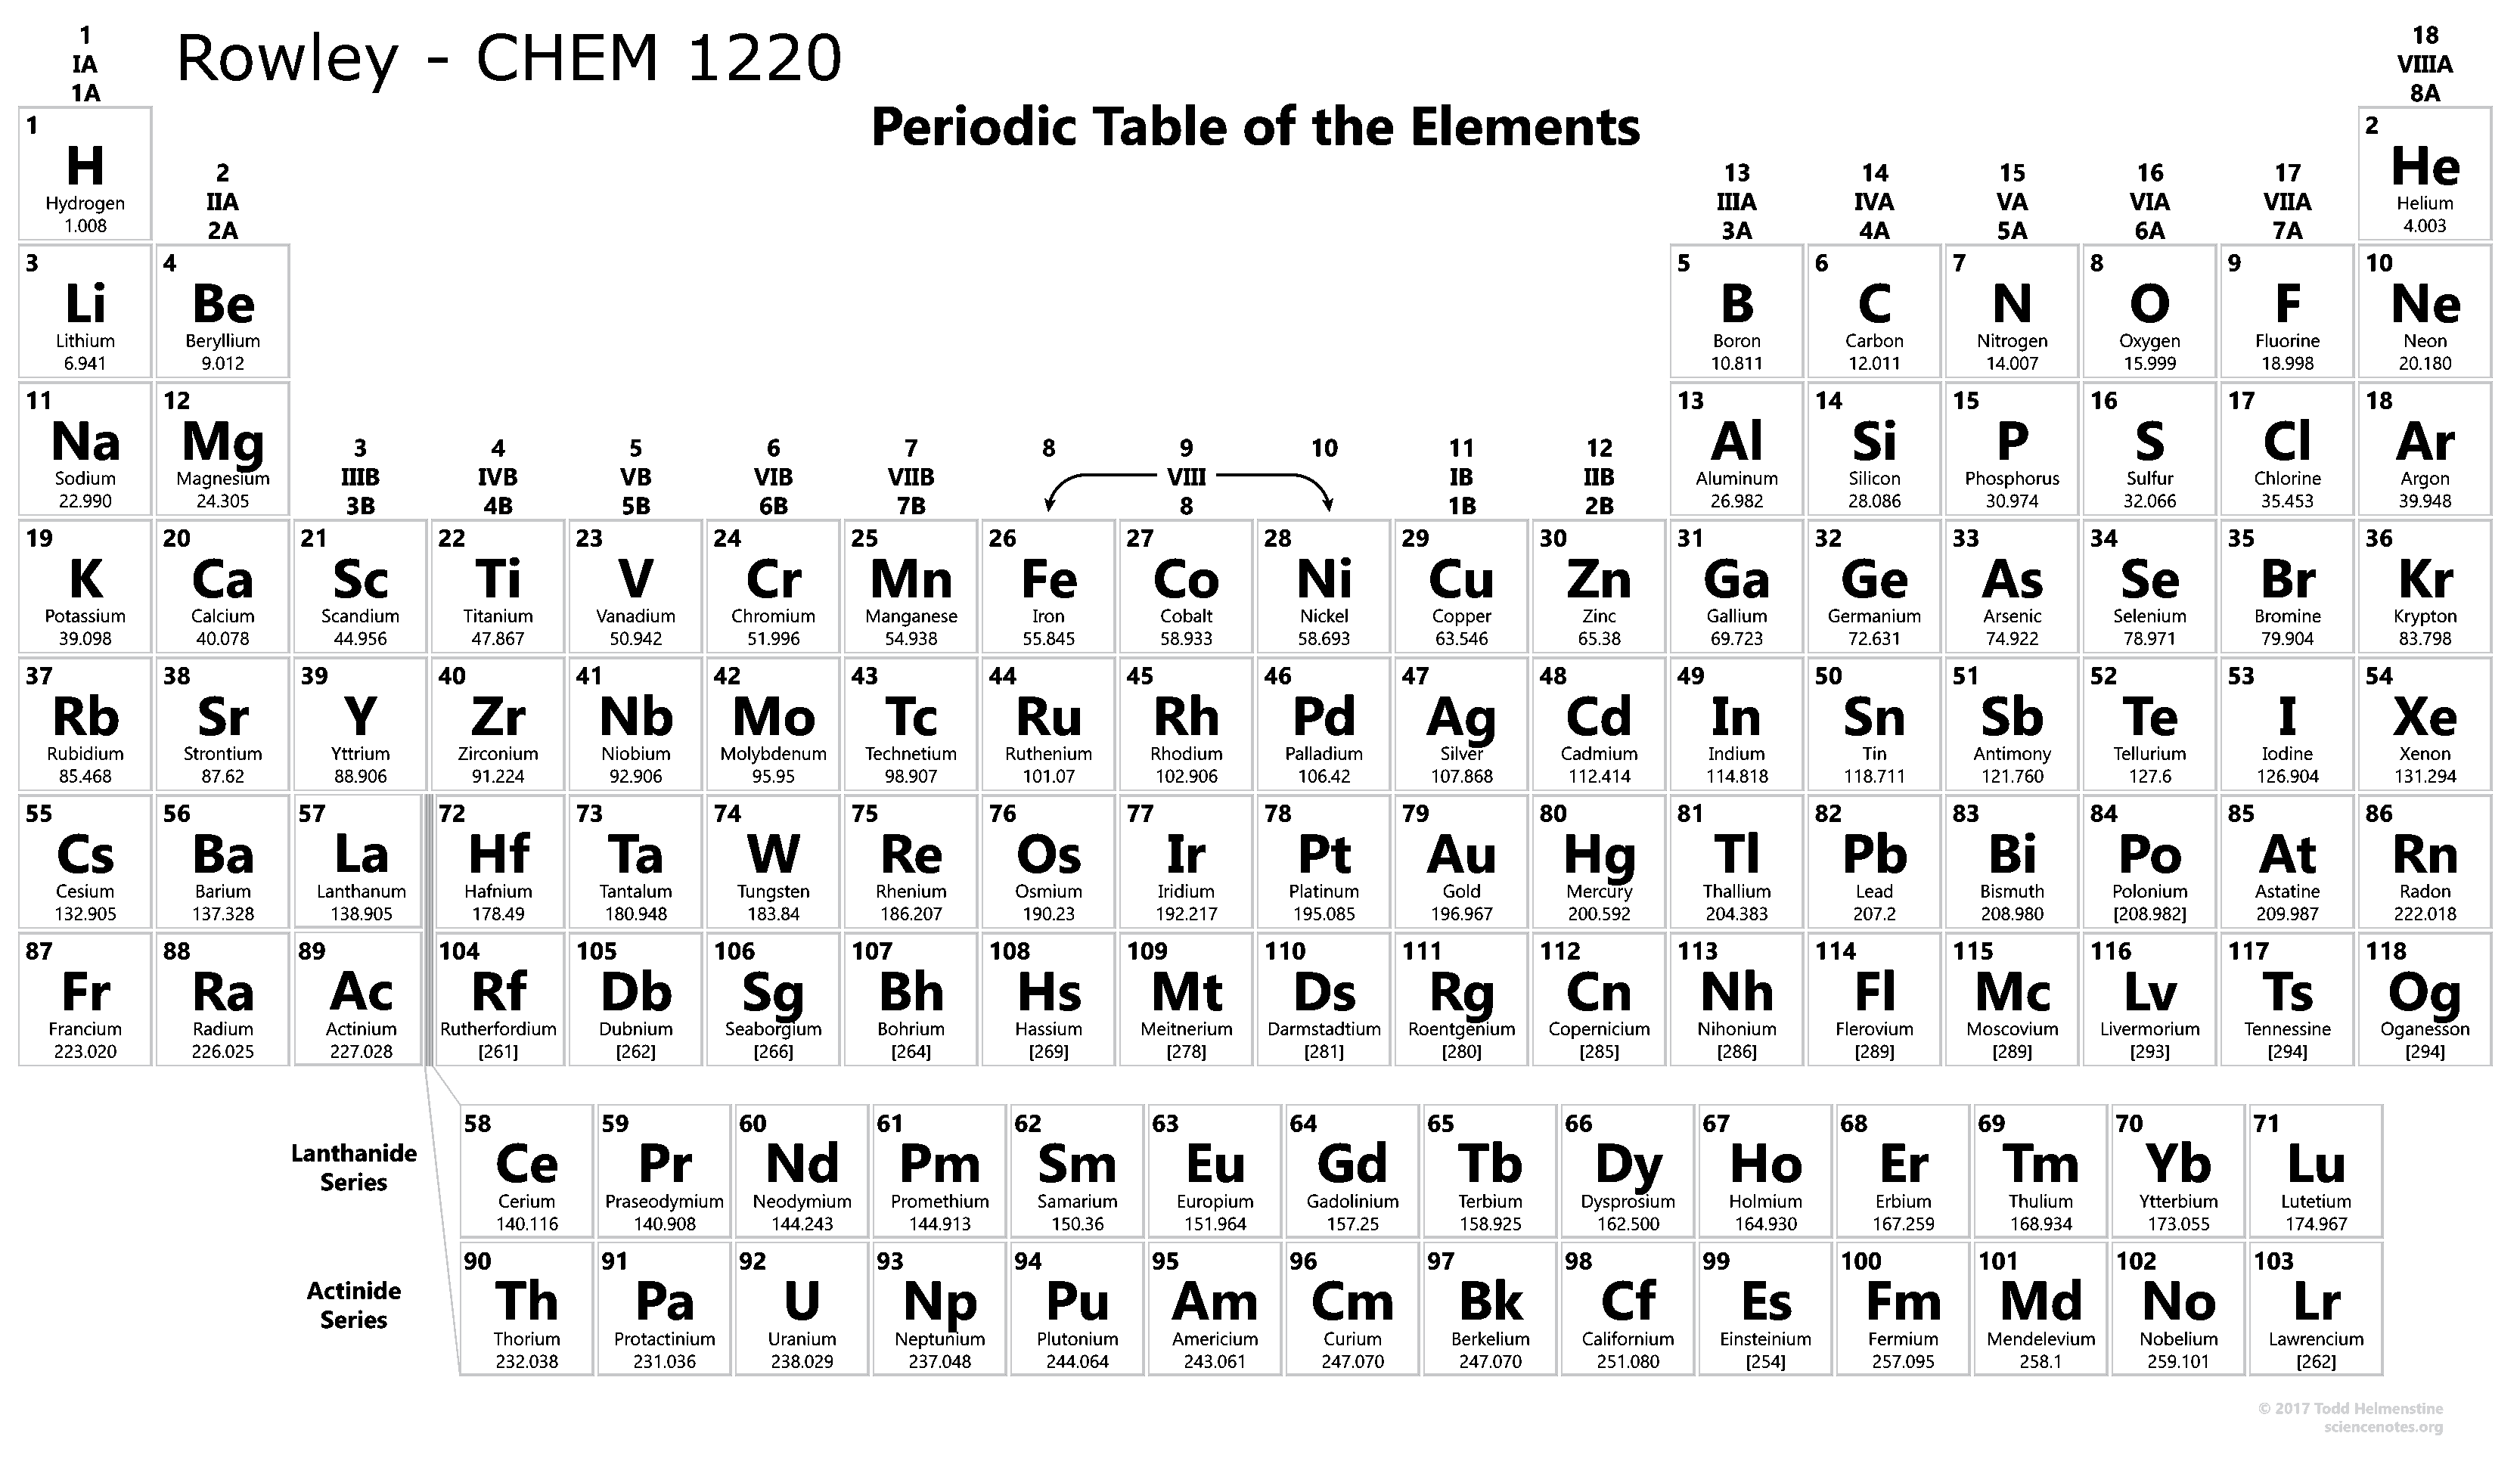
\includegraphics[width=1.3\textwidth, angle =90]{UpdatedTable.png}

	\restoregeometry


\end{document}
